% Options for packages loaded elsewhere
\PassOptionsToPackage{unicode}{hyperref}
\PassOptionsToPackage{hyphens}{url}
%
\documentclass[
  man]{apa6}
\usepackage{amsmath,amssymb}
\usepackage{iftex}
\ifPDFTeX
  \usepackage[T1]{fontenc}
  \usepackage[utf8]{inputenc}
  \usepackage{textcomp} % provide euro and other symbols
\else % if luatex or xetex
  \usepackage{unicode-math} % this also loads fontspec
  \defaultfontfeatures{Scale=MatchLowercase}
  \defaultfontfeatures[\rmfamily]{Ligatures=TeX,Scale=1}
\fi
\usepackage{lmodern}
\ifPDFTeX\else
  % xetex/luatex font selection
\fi
% Use upquote if available, for straight quotes in verbatim environments
\IfFileExists{upquote.sty}{\usepackage{upquote}}{}
\IfFileExists{microtype.sty}{% use microtype if available
  \usepackage[]{microtype}
  \UseMicrotypeSet[protrusion]{basicmath} % disable protrusion for tt fonts
}{}
\makeatletter
\@ifundefined{KOMAClassName}{% if non-KOMA class
  \IfFileExists{parskip.sty}{%
    \usepackage{parskip}
  }{% else
    \setlength{\parindent}{0pt}
    \setlength{\parskip}{6pt plus 2pt minus 1pt}}
}{% if KOMA class
  \KOMAoptions{parskip=half}}
\makeatother
\usepackage{xcolor}
\usepackage{graphicx}
\makeatletter
\def\maxwidth{\ifdim\Gin@nat@width>\linewidth\linewidth\else\Gin@nat@width\fi}
\def\maxheight{\ifdim\Gin@nat@height>\textheight\textheight\else\Gin@nat@height\fi}
\makeatother
% Scale images if necessary, so that they will not overflow the page
% margins by default, and it is still possible to overwrite the defaults
% using explicit options in \includegraphics[width, height, ...]{}
\setkeys{Gin}{width=\maxwidth,height=\maxheight,keepaspectratio}
% Set default figure placement to htbp
\makeatletter
\def\fps@figure{htbp}
\makeatother
\setlength{\emergencystretch}{3em} % prevent overfull lines
\providecommand{\tightlist}{%
  \setlength{\itemsep}{0pt}\setlength{\parskip}{0pt}}
\setcounter{secnumdepth}{-\maxdimen} % remove section numbering
% Make \paragraph and \subparagraph free-standing
\ifx\paragraph\undefined\else
  \let\oldparagraph\paragraph
  \renewcommand{\paragraph}[1]{\oldparagraph{#1}\mbox{}}
\fi
\ifx\subparagraph\undefined\else
  \let\oldsubparagraph\subparagraph
  \renewcommand{\subparagraph}[1]{\oldsubparagraph{#1}\mbox{}}
\fi
\ifLuaTeX
\usepackage[bidi=basic]{babel}
\else
\usepackage[bidi=default]{babel}
\fi
\babelprovide[main,import]{english}
% get rid of language-specific shorthands (see #6817):
\let\LanguageShortHands\languageshorthands
\def\languageshorthands#1{}
% Manuscript styling
\usepackage{upgreek}
\captionsetup{font=singlespacing,justification=justified}

% Table formatting
\usepackage{longtable}
\usepackage{lscape}
% \usepackage[counterclockwise]{rotating}   % Landscape page setup for large tables
\usepackage{multirow}		% Table styling
\usepackage{tabularx}		% Control Column width
\usepackage[flushleft]{threeparttable}	% Allows for three part tables with a specified notes section
\usepackage{threeparttablex}            % Lets threeparttable work with longtable

% Create new environments so endfloat can handle them
% \newenvironment{ltable}
%   {\begin{landscape}\centering\begin{threeparttable}}
%   {\end{threeparttable}\end{landscape}}
\newenvironment{lltable}{\begin{landscape}\centering\begin{ThreePartTable}}{\end{ThreePartTable}\end{landscape}}

% Enables adjusting longtable caption width to table width
% Solution found at http://golatex.de/longtable-mit-caption-so-breit-wie-die-tabelle-t15767.html
\makeatletter
\newcommand\LastLTentrywidth{1em}
\newlength\longtablewidth
\setlength{\longtablewidth}{1in}
\newcommand{\getlongtablewidth}{\begingroup \ifcsname LT@\roman{LT@tables}\endcsname \global\longtablewidth=0pt \renewcommand{\LT@entry}[2]{\global\advance\longtablewidth by ##2\relax\gdef\LastLTentrywidth{##2}}\@nameuse{LT@\roman{LT@tables}} \fi \endgroup}

% \setlength{\parindent}{0.5in}
% \setlength{\parskip}{0pt plus 0pt minus 0pt}

% Overwrite redefinition of paragraph and subparagraph by the default LaTeX template
% See https://github.com/crsh/papaja/issues/292
\makeatletter
\renewcommand{\paragraph}{\@startsection{paragraph}{4}{\parindent}%
  {0\baselineskip \@plus 0.2ex \@minus 0.2ex}%
  {-1em}%
  {\normalfont\normalsize\bfseries\itshape\typesectitle}}

\renewcommand{\subparagraph}[1]{\@startsection{subparagraph}{5}{1em}%
  {0\baselineskip \@plus 0.2ex \@minus 0.2ex}%
  {-\z@\relax}%
  {\normalfont\normalsize\itshape\hspace{\parindent}{#1}\textit{\addperi}}{\relax}}
\makeatother

% \usepackage{etoolbox}
\makeatletter
\patchcmd{\HyOrg@maketitle}
  {\section{\normalfont\normalsize\abstractname}}
  {\section*{\normalfont\normalsize\abstractname}}
  {}{\typeout{Failed to patch abstract.}}
\patchcmd{\HyOrg@maketitle}
  {\section{\protect\normalfont{\@title}}}
  {\section*{\protect\normalfont{\@title}}}
  {}{\typeout{Failed to patch title.}}
\makeatother

\usepackage{xpatch}
\makeatletter
\xapptocmd\appendix
  {\xapptocmd\section
    {\addcontentsline{toc}{section}{\appendixname\ifoneappendix\else~\theappendix\fi\\: #1}}
    {}{\InnerPatchFailed}%
  }
{}{\PatchFailed}
\keywords{keywords\newline\indent Word count: X}
\DeclareDelayedFloatFlavor{ThreePartTable}{table}
\DeclareDelayedFloatFlavor{lltable}{table}
\DeclareDelayedFloatFlavor*{longtable}{table}
\makeatletter
\renewcommand{\efloat@iwrite}[1]{\immediate\expandafter\protected@write\csname efloat@post#1\endcsname{}}
\makeatother
\usepackage{csquotes}
\ifLuaTeX
  \usepackage{selnolig}  % disable illegal ligatures
\fi
\IfFileExists{bookmark.sty}{\usepackage{bookmark}}{\usepackage{hyperref}}
\IfFileExists{xurl.sty}{\usepackage{xurl}}{} % add URL line breaks if available
\urlstyle{same}
\hypersetup{
  pdftitle={The title},
  pdfauthor={First Author1 \& Ernst-August Doelle1,2},
  pdflang={en-EN},
  pdfkeywords={keywords},
  hidelinks,
  pdfcreator={LaTeX via pandoc}}

\title{The title}
\author{First Author\textsuperscript{1} \& Ernst-August Doelle\textsuperscript{1,2}}
\date{}


\shorttitle{Title}

\authornote{

Add complete departmental affiliations for each author here. Each new line herein must be indented, like this line.

Enter author note here.

The authors made the following contributions. First Author: Conceptualization, Writing - Original Draft Preparation, Writing - Review \& Editing; Ernst-August Doelle: Writing - Review \& Editing, Supervision.

Correspondence concerning this article should be addressed to First Author, Postal address. E-mail: \href{mailto:my@email.com}{\nolinkurl{my@email.com}}

}

\affiliation{\vspace{0.5cm}\textsuperscript{1} Wilhelm-Wundt-University\\\textsuperscript{2} Konstanz Business School}

\abstract{%
One or two sentences providing a \textbf{basic introduction} to the field, comprehensible to a scientist in any discipline.
}



\begin{document}
\maketitle

\renewcommand{\arraystretch}{0.65}

\hypertarget{results}{%
\section{Results}\label{results}}

The aggregated data-set describes 314,925 observations of daily physical activity and sleep from 24,935 unique participants. Table \ref{demo-participants} shows demographic information for all participants. A table of study characteristics can be found in supplementary materials.

\begin{table}[tbp]

\begin{center}
\begin{threeparttable}

\caption{\label{tab:demo-participants}Participant characteristics}

\begin{tabular}{ll}
\toprule
Variable & \multicolumn{1}{c}{Value}\\
\midrule
Numeric variables & \\
\ \ \ Valid weartime hours & 18.01 (5.41)\\
\ \ \ PA volume & 39.39 (19.84)\\
\ \ \ PA intensity & -2.34 (0.31)\\
\ \ \ Sleep duration & 387.49 (110.41)\\
\ \ \ Sleep efficiency & 0.77 (0.14)\\
\ \ \ Sleep onset & 22.55 (2.11)\\
\ \ \ Sleep wakeup & 31.11 (1.46)\\
\ \ \ Sleep regularity & 55.03 (12.77)\\
\ \ \ Age & 35.28 (28.33)\\
\ \ \ BMI & 21.74 (5.92)\\
Accelerometer Wear Location & \\
\ \ \ Hip & 8,830 (35.41\%)\\
\ \ \ Wrist & 16,105 (64.59\%)\\
Region & \\
\ \ \ Africa & 1,090 (4.37\%)\\
\ \ \ Asia & \ \  731 (2.93\%)\\
\ \ \ Europe & 14,840 (59.51\%)\\
\ \ \ North america & 1,449 (5.81\%)\\
\ \ \ Oceania & 3,183 (12.77\%)\\
\ \ \ South america & 3,642 (14.61\%)\\
Season & \\
\ \ \ Autumn & 6,644 (26.65\%)\\
\ \ \ Spring & 7,874 (31.58\%)\\
\ \ \ Summer & 4,137 (16.59\%)\\
\ \ \ Winter & 6,280 (25.19\%)\\
Sex & \\
\ \ \ Female & 12,393 (49.70\%)\\
\ \ \ Male & 12,542 (50.30\%)\\
Sleep Conditions Reported & \\
\ \ \ Yes & 1,009 (4.05\%)\\
Socioeconomic Status & \\
\ \ \ Low & 8,375 (33.59\%)\\
\ \ \ Medium & 8,510 (34.13\%)\\
\ \ \ High & 8,050 (32.28\%)\\
\bottomrule
\addlinespace
\end{tabular}

\begin{tablenotes}[para]
\normalsize{\textit{Note.} For categorical variables the value is the count, and percentage. For numeric variables the value is the Mean and SD. N = 24,935}
\end{tablenotes}

\end{threeparttable}
\end{center}

\end{table}

\hypertarget{the-effects-of-physical-activity-volume-on-sleep}{%
\subsection{The effects of physical activity volume on sleep}\label{the-effects-of-physical-activity-volume-on-sleep}}

We estimated the effects of physical activity on sleep (RQ1) using mixed-effects models. We estimated the effect of physical activity volume on sleep by age, and the results are presented in Table \ref{tab:sleep-by-volume} and Figure \ref{fig:sleep-by-volume-fig}. There was no meaningful relationship between physical activity volume and sleep duration. However, we observed a curvilinear relationships between physical activity volume and sleep efficiency, onset, and regularity, all of which interacted with age. Sleep efficiency improved with greater physical activity volume, but improvements tapered off for older individuals. Physical activity volume and sleep onset had a positive association for younger individuals, but a negative association for older individuals, where sleep onset was reduced among those with the highest physical activity. There was a strong positive association between physical activity volume and sleep regularity, which was strongest among older participants. For participants aged 35 years and above, this link weakened among those with a physical activity volume greater than two standard deviations.

\begin{table}[tbp]

\begin{center}
\begin{threeparttable}

\caption{\label{tab:sleep-by-volume}Sleep on physical activity volume controlling for SES, gender and BMI}

\begin{tabular}{lllll}
\toprule
Term & \multicolumn{1}{c}{$\beta$ [95\% CI]} & \multicolumn{1}{c}{SE} & \multicolumn{1}{c}{t} & \multicolumn{1}{c}{p}\\
\midrule
Sleep duration &  &  &  & \\
\ \ \ (Intercept) & -0.23 [-0.55, 0.10] & 0.17 & -1.37 & .189\\
\ \ \ Scale PA volume & 0.02 [-0.04, 0.08] & 0.03 & 0.68 & .528\\
\ \ \ Age & 0.00 [0.00, 0.00] & 0.00 & -1.20 & .231\\
\ \ \ Scale PA volume$^2$ & 0.00 [-0.01, 0.02] & 0.01 & 0.55 & .593\\
\ \ \ Scale PA volume:age & 0.00 [0.00, 0.00] & 0.00 & 1.20 & .249\\
\ \ \ Age:scale PA volume$^2$ & 0.00 [0.00, 0.00] & 0.00 & -0.89 & .399\\
Sleep efficiency &  &  &  & \\
\ \ \ (Intercept) & -1.03 [-1.51, -0.54] & 0.25 & -4.15 & .005\\
\ \ \ Scale PA volume & 0.20 [0.16, 0.24] & 0.02 & 10.34 & < .001\\
\ \ \ Age & 0.01 [0.01, 0.01] & 0.00 & 9.72 & .003\\
\ \ \ Scale PA volume$^2$ & -0.02 [-0.03, -0.01] & 0.01 & -3.04 & .005\\
\ \ \ Scale PA volume:age & 0.00 [0.00, 0.00] & 0.00 & -3.07 & .005\\
\ \ \ Age:scale PA volume$^2$ & 0.00 [0.00, 0.00] & 0.00 & -0.54 & .618\\
Sleep onset &  &  &  & \\
\ \ \ (Intercept) & -1.01 [-1.15, -0.87] & 0.07 & -14.16 & < .001\\
\ \ \ Scale PA volume & 0.13 [0.10, 0.16] & 0.02 & 7.65 & < .001\\
\ \ \ Age & 0.02 [0.02, 0.02] & 0.00 & 32.14 & < .001\\
\ \ \ Scale PA volume$^2$ & -0.02 [-0.03, 0.00] & 0.01 & -2.78 & .048\\
\ \ \ Scale PA volume:age & 0.00 [0.00, 0.00] & 0.00 & -8.47 & < .001\\
\ \ \ Age:scale PA volume$^2$ & 0.00 [0.00, 0.00] & 0.00 & 1.61 & .179\\
Sleep regularity &  &  &  & \\
\ \ \ (Intercept) & -0.05 [-0.29, 0.18] & 0.12 & -0.43 & .697\\
\ \ \ Scale PA volume & 0.33 [0.29, 0.37] & 0.02 & 17.05 & < .001\\
\ \ \ Age & 0.01 [0.00, 0.01] & 0.00 & 4.53 & .032\\
\ \ \ Scale PA volume$^2$ & -0.03 [-0.04, -0.02] & 0.00 & -6.18 & < .001\\
\ \ \ Scale PA volume:age & 0.00 [0.00, 0.00] & 0.00 & 0.71 & .486\\
\ \ \ Age:scale PA volume$^2$ & 0.00 [0.00, 0.00] & 0.00 & -3.87 & < .001\\
\bottomrule
\addlinespace
\end{tabular}

\begin{tablenotes}[para]
\normalsize{\textit{Note.} Adjusted for SES, BMI, and sex. }
\end{tablenotes}

\end{threeparttable}
\end{center}

\end{table}

\begin{figure}
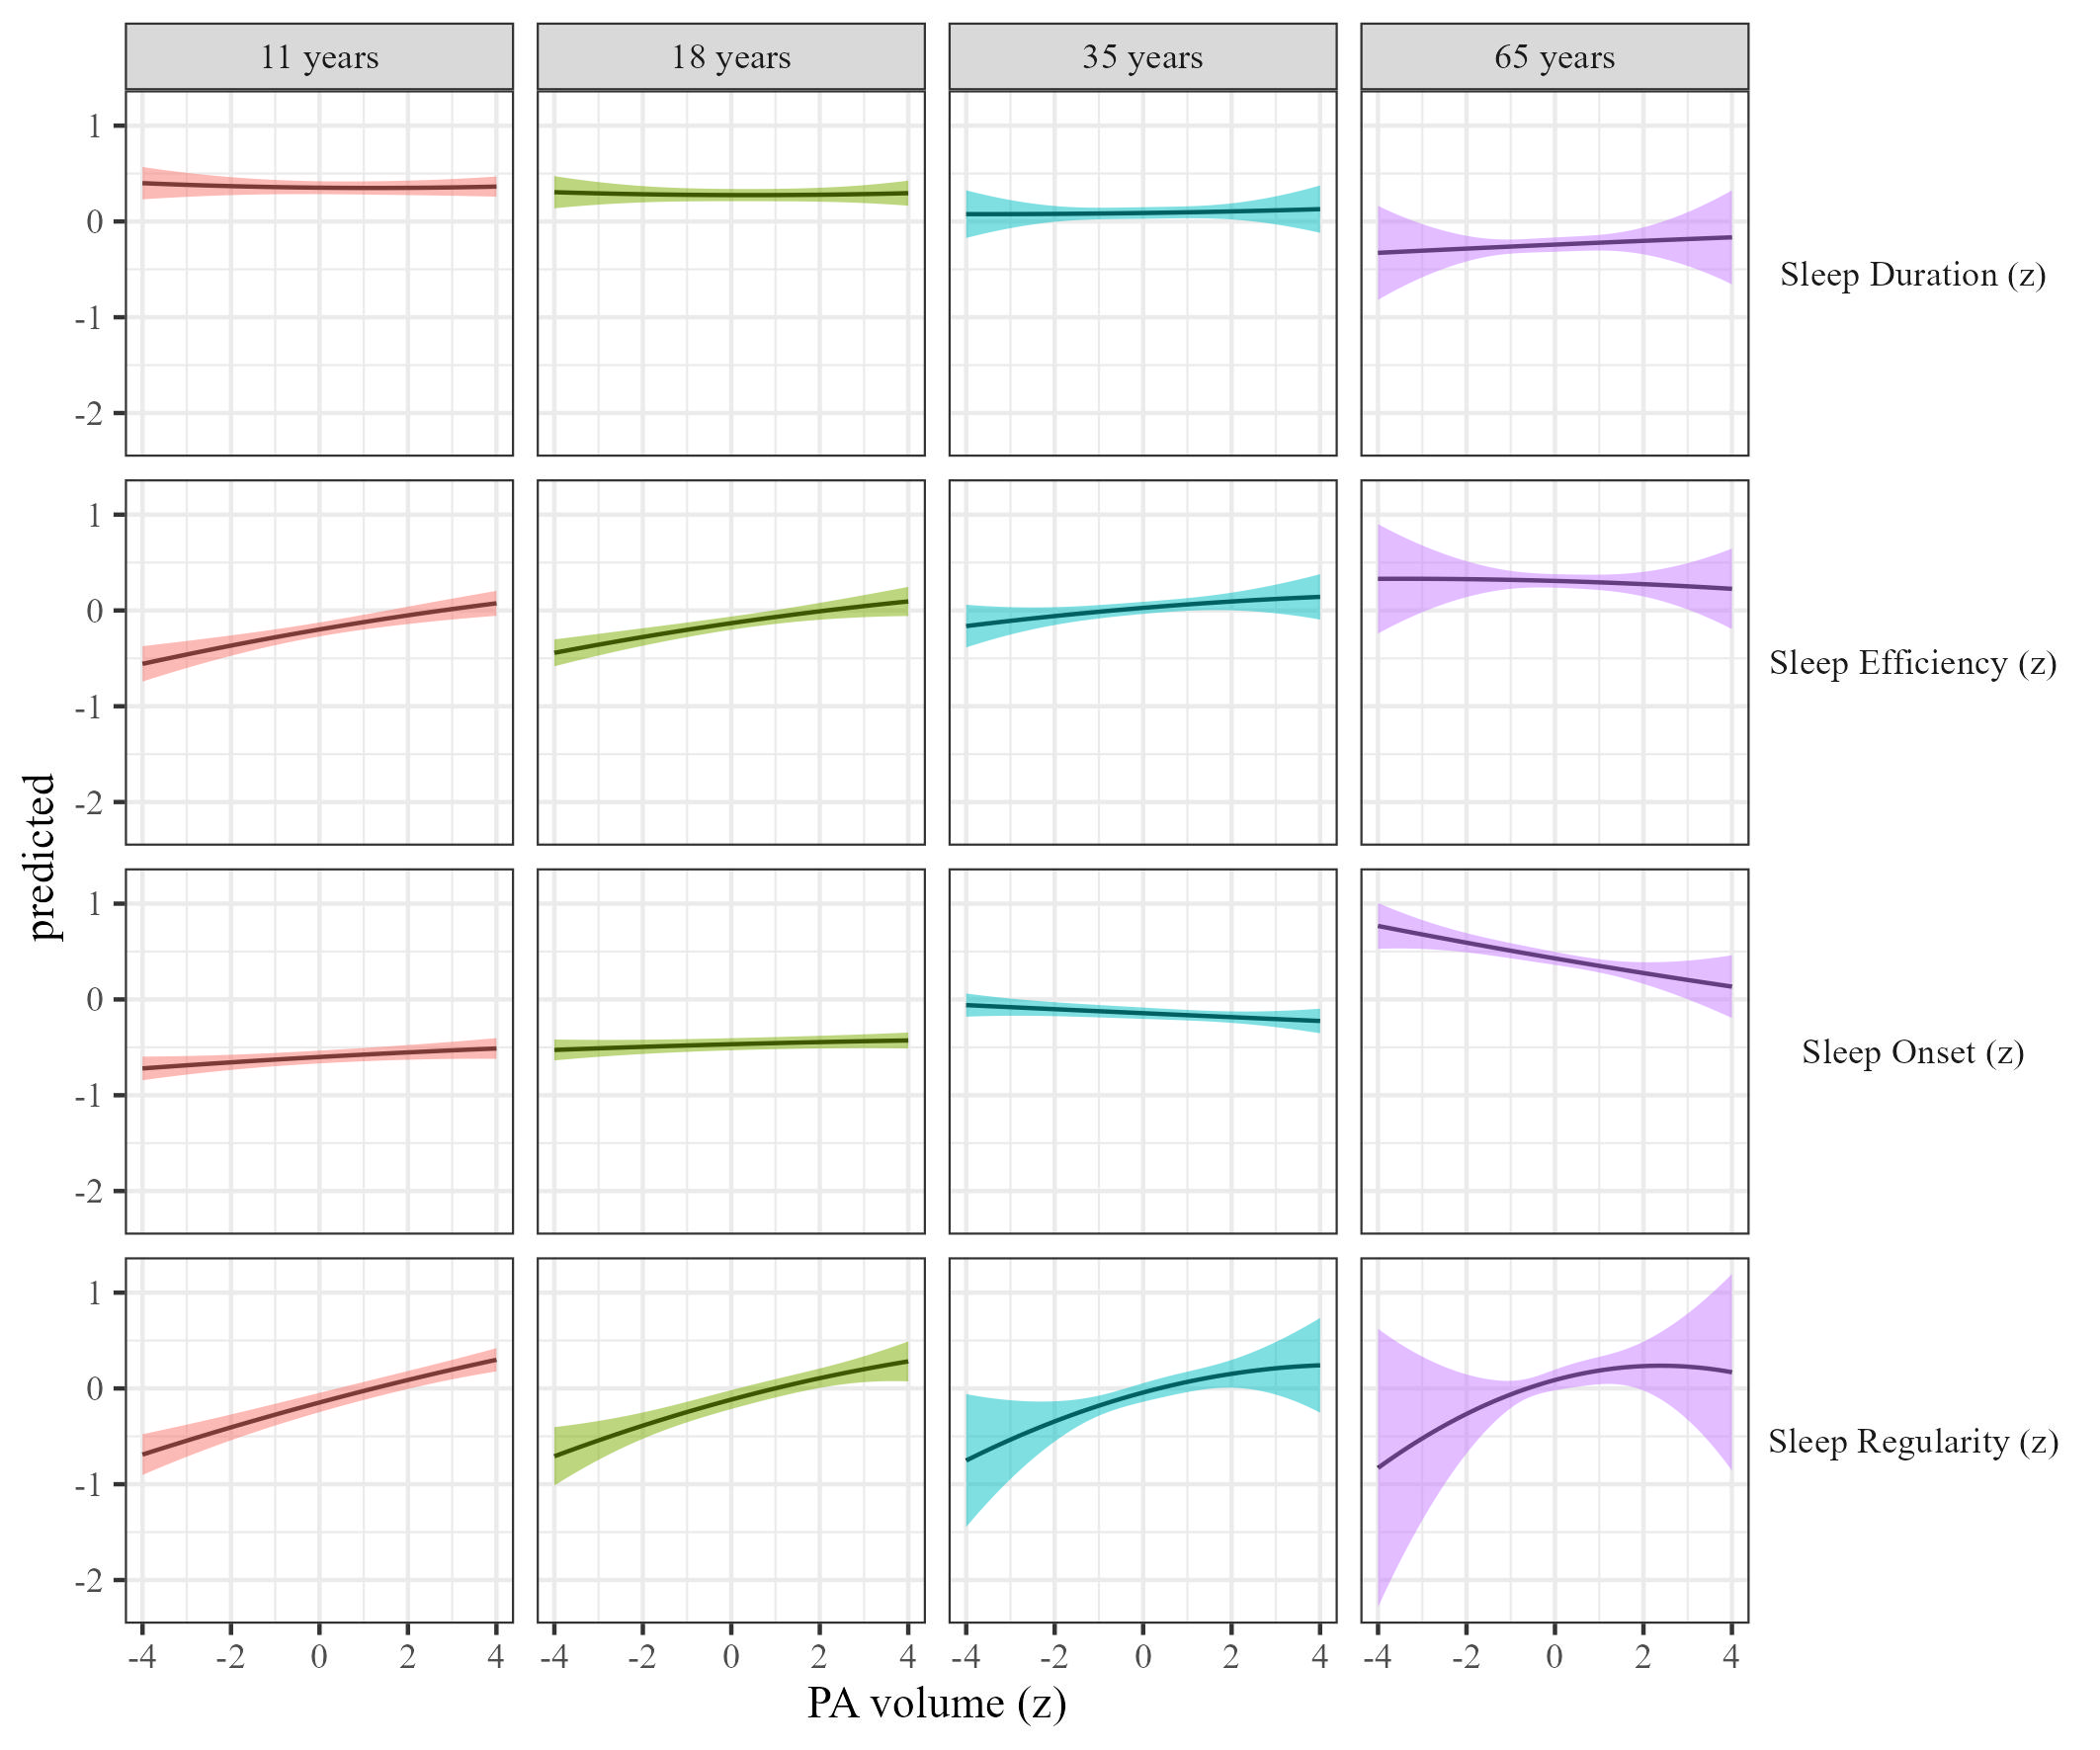
\includegraphics[width=1.1\linewidth]{../Figures/sleep on pa_volume} \caption{Sleep metrics on Physical activity volume}\label{fig:sleep-by-volume-fig}
\end{figure}

\hypertarget{the-effects-of-physical-activity-intensity-on-sleep}{%
\subsection{The effects of physical activity intensity on sleep}\label{the-effects-of-physical-activity-intensity-on-sleep}}

We estimated how physical activity intensity affects sleep across different age groups. We present the results controlling for sex, SES, and BMI, in Table \ref{tab:sleep-by-intensity} and Figure \ref{fig:sleep-by-intensity-fig}. We found that higher physical activity intensity is directly proportional to longer sleep duration and better sleep efficiency. In the case of older participants, physical activity intensity had a U-shaped relationship with sleep onset, meaning that individuals with very low or very high physical activity intensity had longer sleep onset. We also found a strong link between physical activity intensity and improved sleep regularity, which weakened at higher intensity levels.

\begin{table}[tbp]

\begin{center}
\begin{threeparttable}

\caption{\label{tab:sleep-by-intensity}Sleep on physical activity intensity controlling for SES, gender and BMI}

\begin{tabular}{lllll}
\toprule
Term & \multicolumn{1}{c}{$\beta$ [95\% CI]} & \multicolumn{1}{c}{SE} & \multicolumn{1}{c}{t} & \multicolumn{1}{c}{p}\\
\midrule
Sleep duration &  &  &  & \\
\ \ \ (Intercept) & -0.26 [-0.60, 0.09] & 0.18 & -1.46 & .171\\
\ \ \ Scale PA intensity & 0.07 [0.03, 0.12] & 0.02 & 3.23 & .001\\
\ \ \ Age & 0.00 [0.00, 0.00] & 0.00 & 0.03 & .978\\
\ \ \ Scale PA intensity$^2$ & -0.01 [-0.04, 0.02] & 0.02 & -0.53 & .596\\
\ \ \ Scale PA intensity:age & 0.00 [0.00, 0.00] & 0.00 & -1.51 & .130\\
\ \ \ Age:scale PA intensity$^2$ & 0.00 [0.00, 0.00] & 0.00 & -0.58 & .565\\
Sleep efficiency &  &  &  & \\
\ \ \ (Intercept) & -1.09 [-1.61, -0.57] & 0.27 & -4.11 & .007\\
\ \ \ Scale PA intensity & 0.08 [0.02, 0.14] & 0.03 & 2.55 & .030\\
\ \ \ Age & 0.01 [0.01, 0.02] & 0.00 & 8.36 & .006\\
\ \ \ Scale PA intensity$^2$ & 0.00 [-0.03, 0.04] & 0.02 & 0.17 & .863\\
\ \ \ Scale PA intensity:age & 0.00 [0.00, 0.00] & 0.00 & -1.32 & .220\\
\ \ \ Age:scale PA intensity$^2$ & 0.00 [0.00, 0.00] & 0.00 & -1.00 & .325\\
Sleep onset &  &  &  & \\
\ \ \ (Intercept) & -0.98 [-1.15, -0.81] & 0.09 & -11.35 & .001\\
\ \ \ Scale PA intensity & -0.03 [-0.07, 0.01] & 0.02 & -1.33 & .213\\
\ \ \ Age & 0.02 [0.02, 0.02] & 0.00 & 28.96 & < .001\\
\ \ \ Scale PA intensity$^2$ & -0.01 [-0.04, 0.01] & 0.01 & -1.09 & .293\\
\ \ \ Scale PA intensity:age & 0.00 [0.00, 0.00] & 0.00 & -0.49 & .627\\
\ \ \ Age:scale PA intensity$^2$ & 0.00 [0.00, 0.00] & 0.00 & 2.45 & .032\\
Sleep regularity &  &  &  & \\
\ \ \ (Intercept) & -0.15 [-0.31, 0.02] & 0.08 & -1.75 & .126\\
\ \ \ Scale PA intensity & 0.28 [0.22, 0.34] & 0.03 & 9.38 & < .001\\
\ \ \ Age & 0.01 [0.01, 0.01] & 0.00 & 5.33 & .019\\
\ \ \ Scale PA intensity$^2$ & -0.04 [-0.07, -0.01] & 0.01 & -2.73 & .010\\
\ \ \ Scale PA intensity:age & 0.00 [0.00, 0.00] & 0.00 & -4.61 & .001\\
\ \ \ Age:scale PA intensity$^2$ & 0.00 [0.00, 0.00] & 0.00 & 0.24 & .810\\
\bottomrule
\addlinespace
\end{tabular}

\begin{tablenotes}[para]
\normalsize{\textit{Note.} Adjusted for SES, BMI, and sex. }
\end{tablenotes}

\end{threeparttable}
\end{center}

\end{table}

\begin{figure}
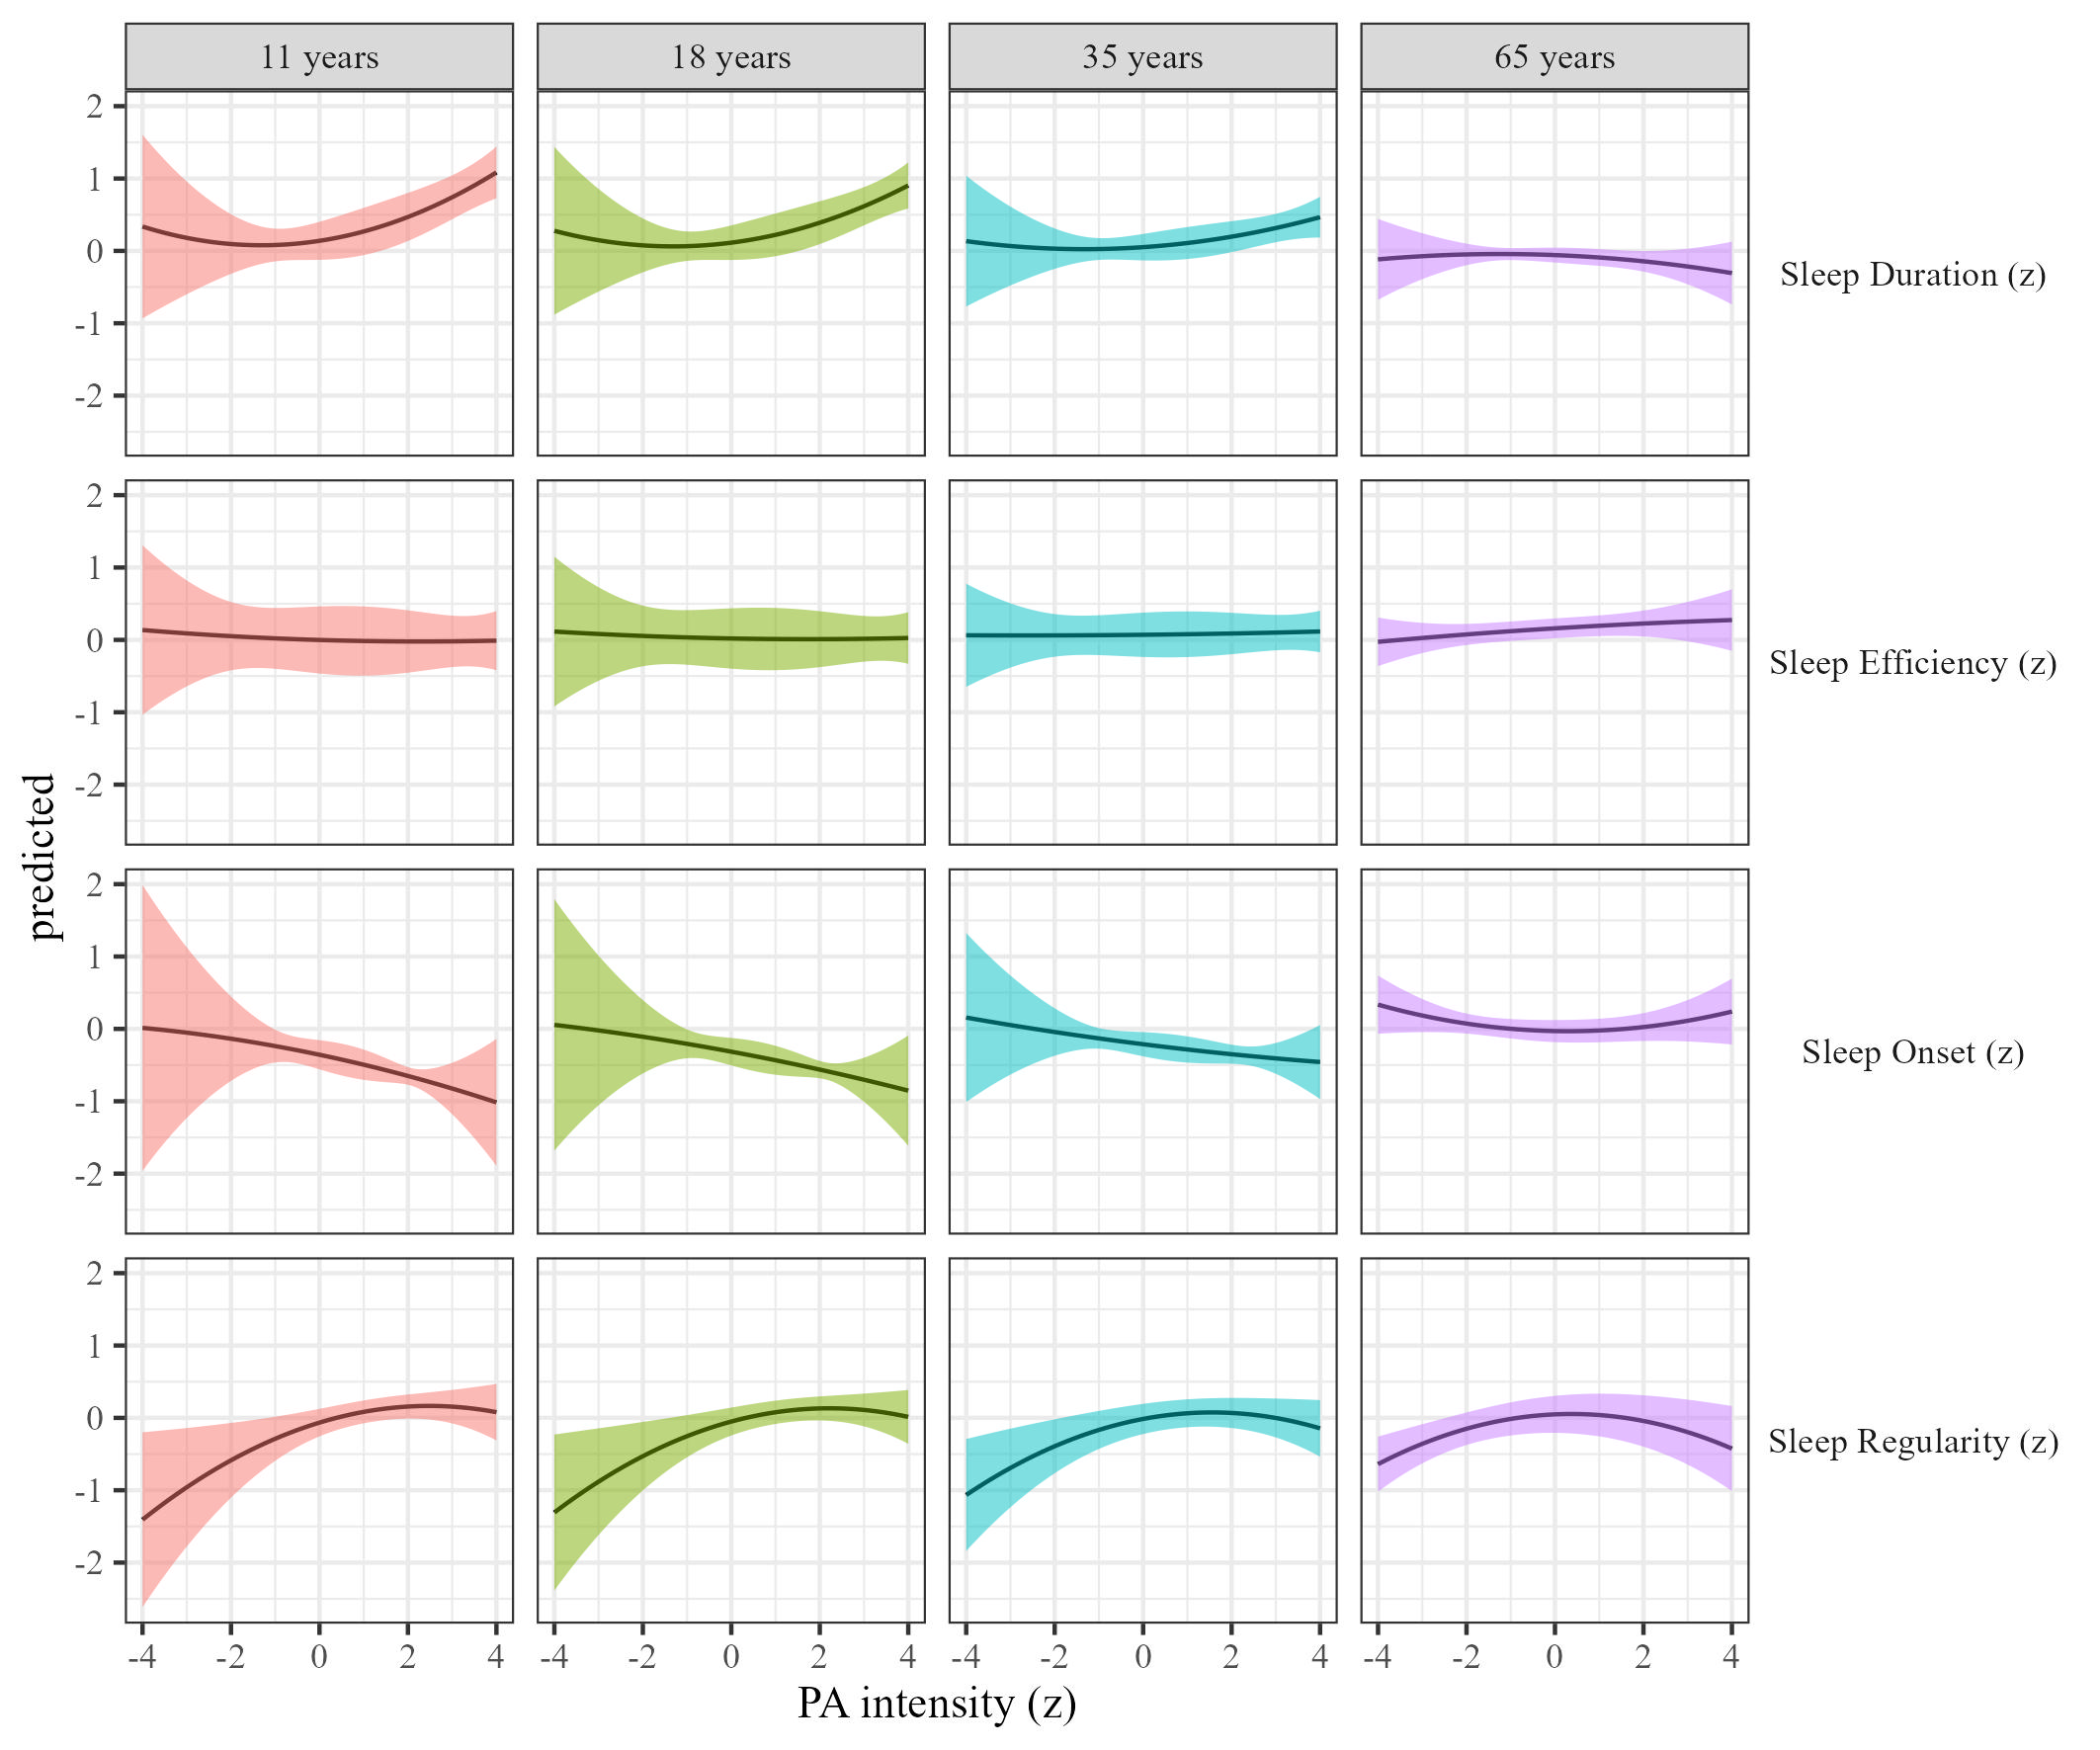
\includegraphics[width=1.1\linewidth]{../Figures/sleep on pa_intensity} \caption{Sleep metrics on Physical activity intensity}\label{fig:sleep-by-intensity-fig}
\end{figure}

\hypertarget{the-effects-of-sleep-duration-on-physical-activity}{%
\subsection{The effects of sleep duration on physical activity}\label{the-effects-of-sleep-duration-on-physical-activity}}

We estimated the effect of sleep duration on physical activity by age. Results, controlling for sex, SES, and BMI are presented in Table \ref{tab:PA-by-sleep-duration} and Figure \ref{fig:PA-by-sleep-duration-fig}. As age increases, both physical activity volume and intensity decrease. We found a subtle inverted U-shaped relationship between average sleep duration and physical activity volume, where the highest volume of physical activity was linked to average sleep duration.

\begin{table}[tbp]

\begin{center}
\begin{threeparttable}

\caption{\label{tab:PA-by-sleep-duration}Physical activity  by sleep duration controlling for SES, gender and BMI}

\begin{tabular}{lllll}
\toprule
Term & \multicolumn{1}{c}{$\beta$ [95\% CI]} & \multicolumn{1}{c}{SE} & \multicolumn{1}{c}{t} & \multicolumn{1}{c}{p}\\
\midrule
PA volume &  &  &  & \\
\ \ \ (Intercept) & 0.44 [0.06, 0.82] & 0.20 & 2.25 & .133\\
\ \ \ Scale sleep duration lag & 0.00 [-0.03, 0.03] & 0.01 & 0.00 & .997\\
\ \ \ Age & -0.01 [-0.01, -0.01] & 0.00 & -6.56 & .004\\
\ \ \ Scale sleep duration lag$^2$ & -0.02 [-0.03, 0.00] & 0.01 & -2.58 & .024\\
\ \ \ Scale sleep duration lag:age & 0.00 [0.00, 0.00] & 0.00 & -1.21 & .251\\
\ \ \ Age:scale sleep duration lag$^2$ & 0.00 [0.00, 0.00] & 0.00 & 0.53 & .596\\
PA intensity &  &  &  & \\
\ \ \ (Intercept) & 0.99 [0.60, 1.37] & 0.20 & 5.01 & .032\\
\ \ \ Scale sleep duration lag & 0.02 [-0.01, 0.05] & 0.02 & 1.18 & .292\\
\ \ \ Age & -0.02 [-0.03, -0.02] & 0.00 & -20.12 & .001\\
\ \ \ Scale sleep duration lag$^2$ & 0.00 [-0.01, 0.01] & 0.01 & -0.64 & .526\\
\ \ \ Scale sleep duration lag:age & 0.00 [0.00, 0.00] & 0.00 & -0.02 & .987\\
\ \ \ Age:scale sleep duration lag$^2$ & 0.00 [0.00, 0.00] & 0.00 & -1.13 & .259\\
\bottomrule
\addlinespace
\end{tabular}

\begin{tablenotes}[para]
\normalsize{\textit{Note.} Adjusted for SES, BMI, and sex. }
\end{tablenotes}

\end{threeparttable}
\end{center}

\end{table}

\begin{figure}
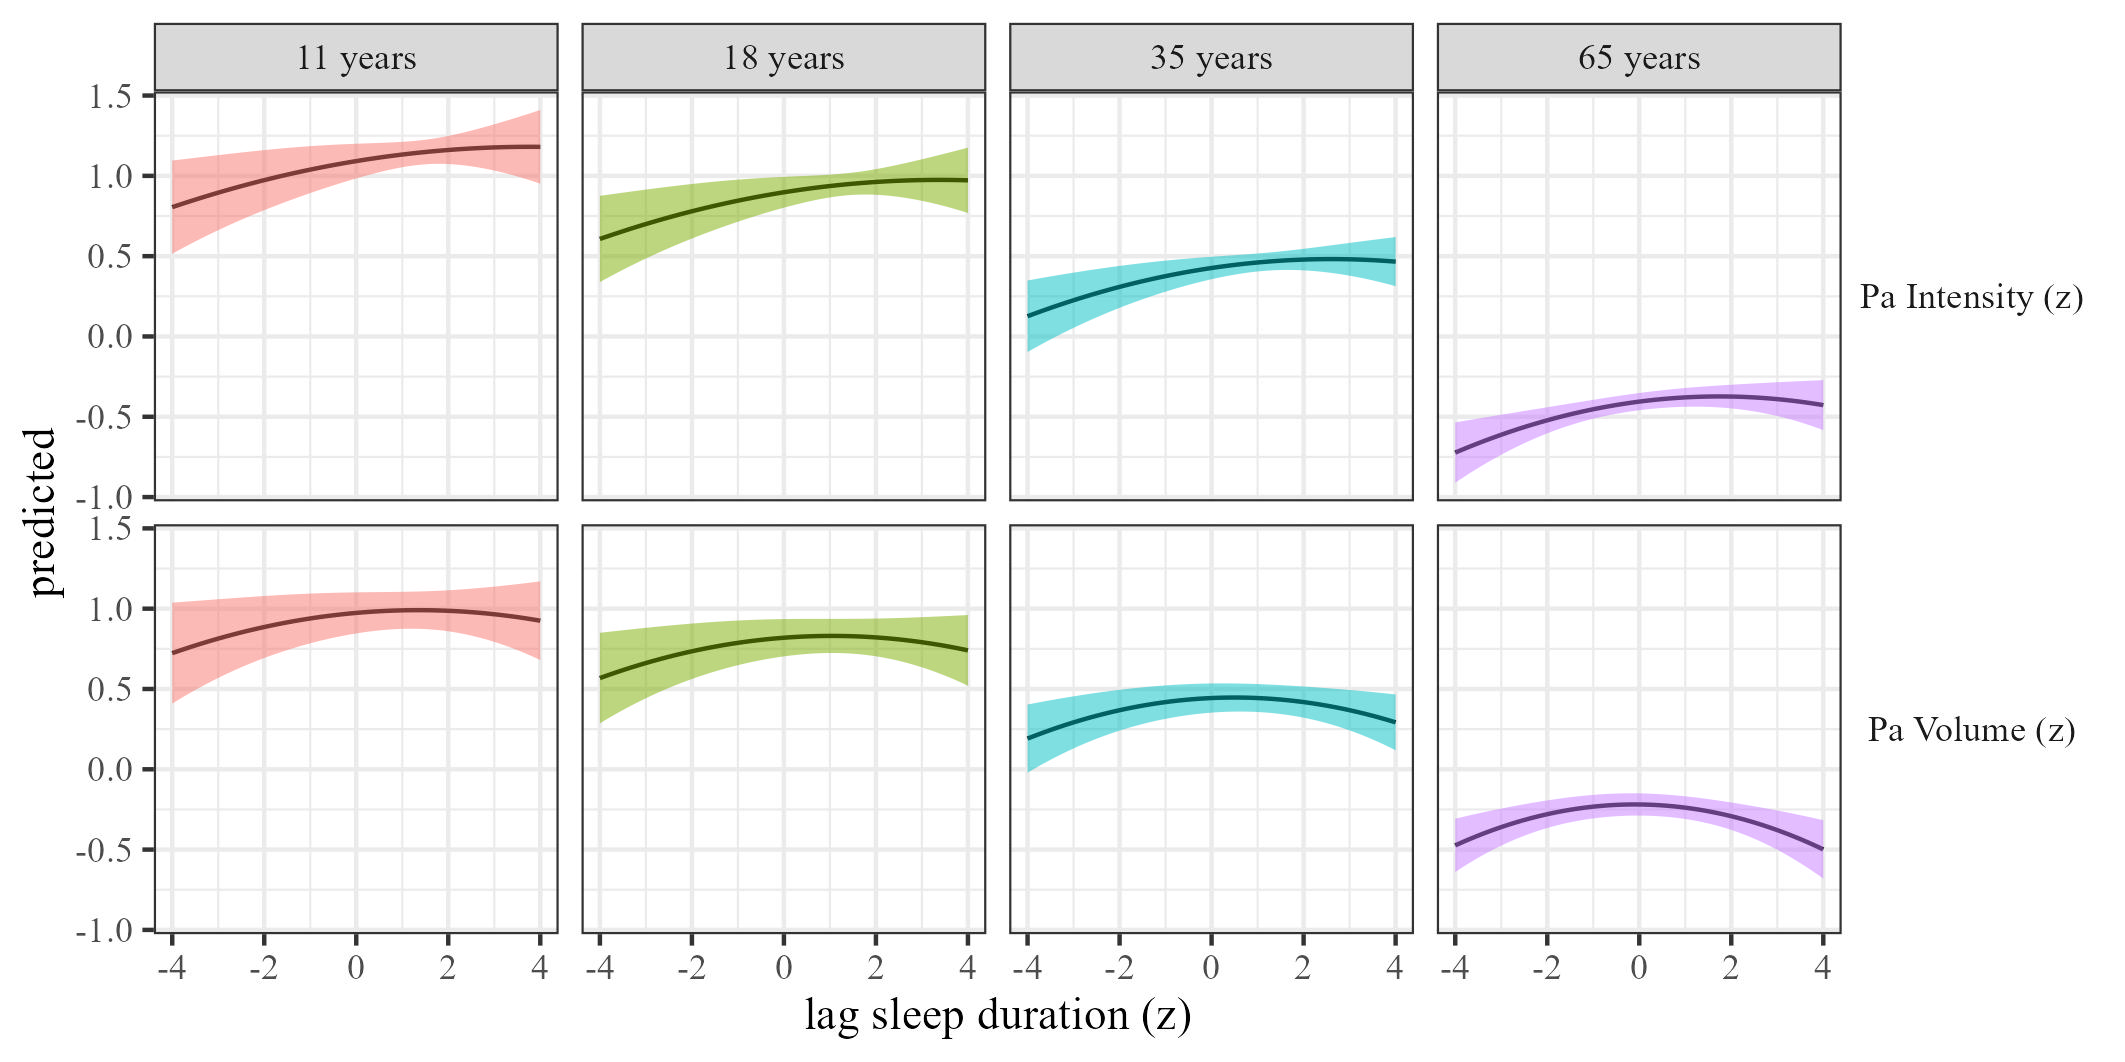
\includegraphics[width=1.1\linewidth]{../Figures/Pa on sleep_duration_lag} \caption{Physical activty by sleep duration}\label{fig:PA-by-sleep-duration-fig}
\end{figure}

\hypertarget{the-effects-of-sleep-efficiency-on-physical-activity}{%
\subsection{The effects of sleep efficiency on physical activity}\label{the-effects-of-sleep-efficiency-on-physical-activity}}

We estimated the effect of sleep efficiency on physical activity by age. Results, controlling for sex, SES, and BMI are presented in Table \ref{tab:PA-by-sleep-efficiency} and Figure \ref{fig:PA-by-sleep-efficiency-fig}. We did not find a relationship between physical activity volume and sleep efficiency. However, there was a subtle U-shaped relationship where individuals with above-average sleep efficiency engaged in more intense physical activity.

\begin{table}[tbp]

\begin{center}
\begin{threeparttable}

\caption{\label{tab:PA-by-sleep-efficiency}Physical activity by sleep efficiency controlling for SES, gender and BMI}

\begin{tabular}{lllll}
\toprule
Term & \multicolumn{1}{c}{$\beta$ [95\% CI]} & \multicolumn{1}{c}{SE} & \multicolumn{1}{c}{t} & \multicolumn{1}{c}{p}\\
\midrule
PA volume &  &  &  & \\
\ \ \ (Intercept) & 0.42 [0.03, 0.81] & 0.20 & 2.11 & .151\\
\ \ \ Scale sleep efficiency lag & 0.04 [-0.02, 0.10] & 0.03 & 1.44 & .238\\
\ \ \ Age & -0.01 [-0.01, -0.01] & 0.00 & -6.63 & .004\\
\ \ \ Scale sleep efficiency lag$^2$ & 0.01 [0.00, 0.02] & 0.01 & 1.23 & .270\\
\ \ \ Scale sleep efficiency lag:age & 0.00 [0.00, 0.00] & 0.00 & -0.77 & .467\\
\ \ \ Age:scale sleep efficiency lag$^2$ & 0.00 [0.00, 0.00] & 0.00 & -0.23 & .815\\
PA intensity &  &  &  & \\
\ \ \ (Intercept) & 0.99 [0.60, 1.37] & 0.20 & 5.03 & .032\\
\ \ \ Scale sleep efficiency lag & 0.03 [0.00, 0.07] & 0.02 & 2.05 & .058\\
\ \ \ Age & -0.02 [-0.03, -0.02] & 0.00 & -19.00 & .001\\
\ \ \ Scale sleep efficiency lag$^2$ & 0.01 [0.00, 0.02] & 0.00 & 2.39 & .019\\
\ \ \ Scale sleep efficiency lag:age & 0.00 [0.00, 0.00] & 0.00 & -0.62 & .544\\
\ \ \ Age:scale sleep efficiency lag$^2$ & 0.00 [0.00, 0.00] & 0.00 & -0.87 & .393\\
\bottomrule
\addlinespace
\end{tabular}

\begin{tablenotes}[para]
\normalsize{\textit{Note.} Adjusted for SES, BMI, and sex. }
\end{tablenotes}

\end{threeparttable}
\end{center}

\end{table}

\begin{figure}
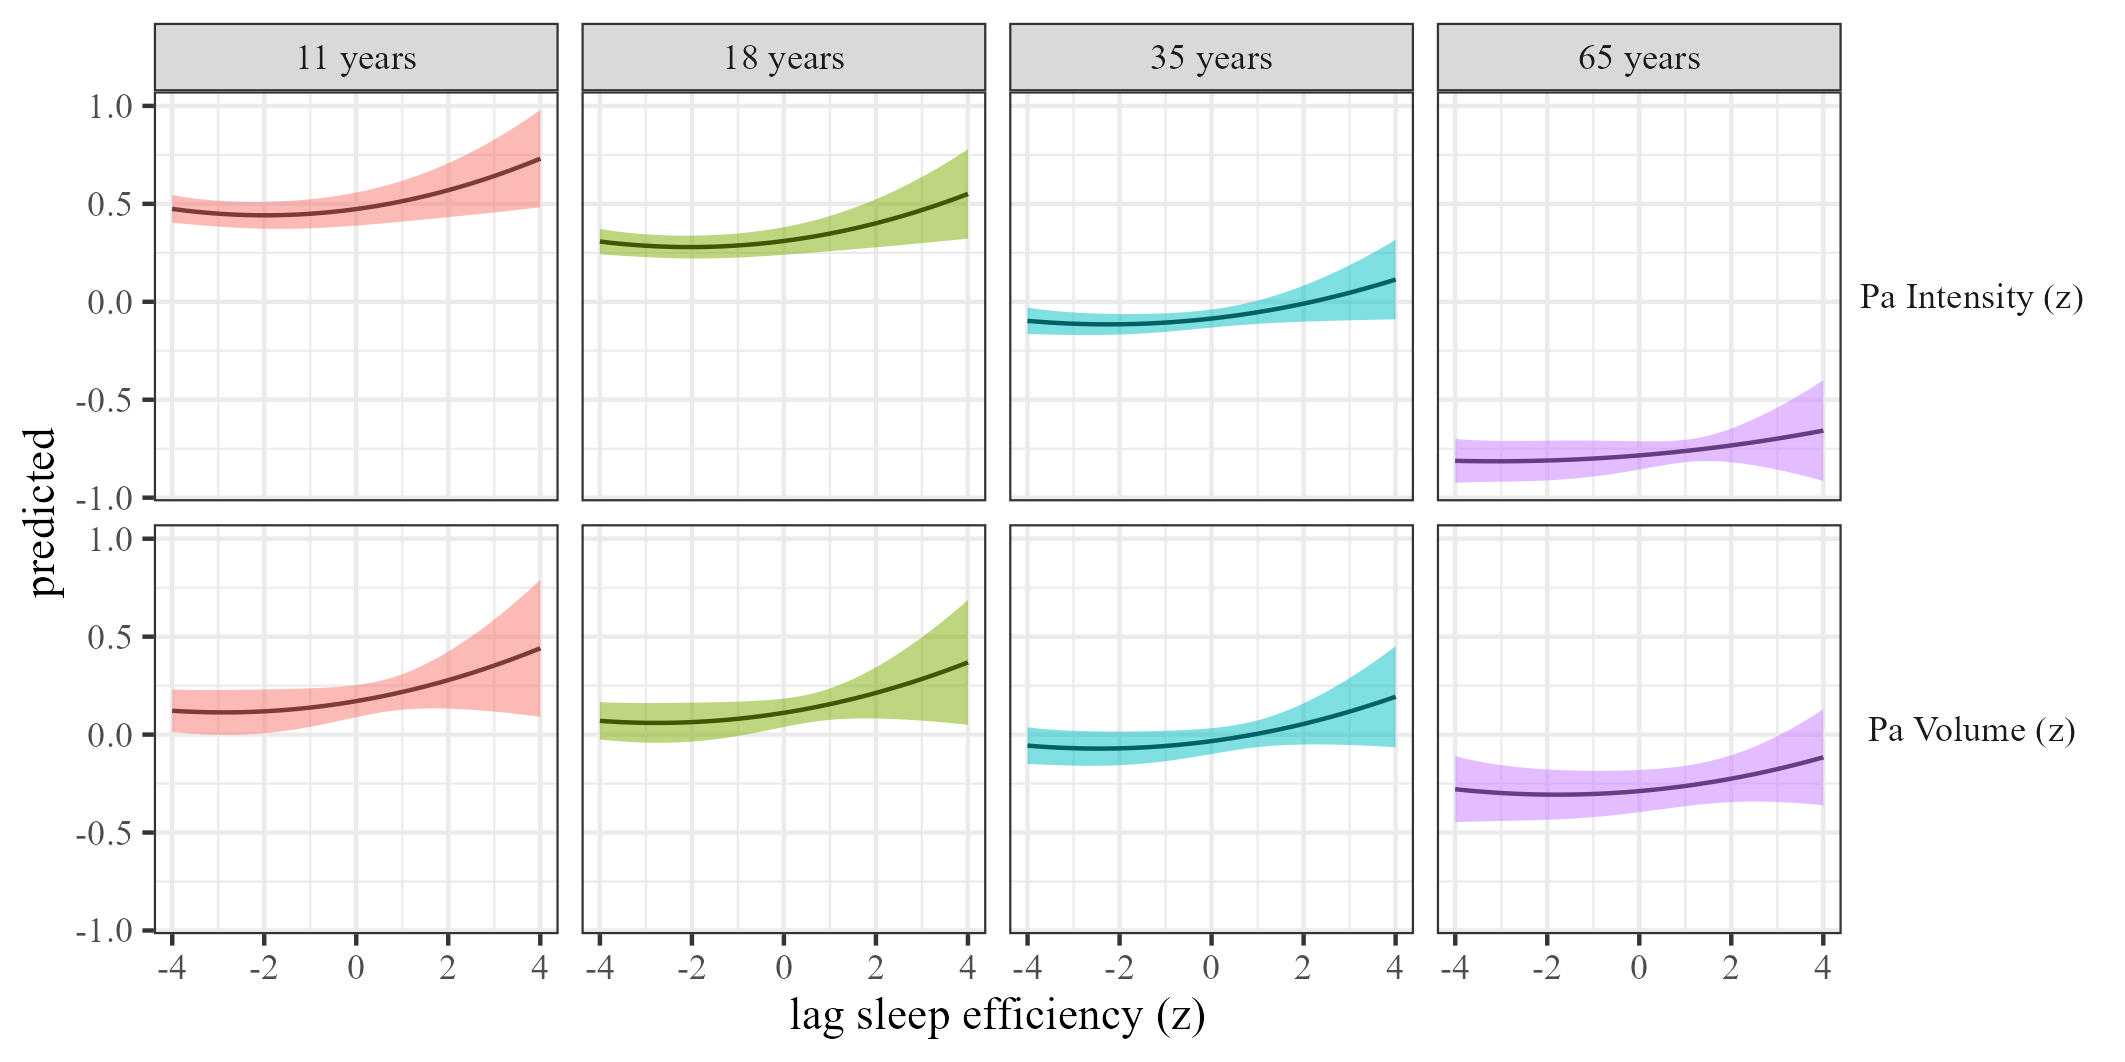
\includegraphics[width=1.1\linewidth]{../Figures/Pa on sleep_efficiency_lag} \caption{Physical activty by sleep efficiency}\label{fig:PA-by-sleep-efficiency-fig}
\end{figure}

\hypertarget{the-effects-of-sleep-onset-on-physical-activity}{%
\subsection{The effects of sleep onset on physical activity}\label{the-effects-of-sleep-onset-on-physical-activity}}

We estimated the effect of sleep onset on physical activity by age. Results, controlling for sex, SES, and BMI are presented in Table \ref{tab:PA-by-sleep-onset} and Figure \ref{fig:PA-by-sleep-onset-fig}. There were strong U-shaped relationships where average sleep onset was linked to the highest levels of physical activity volume and intensity. The U-shaped relationship between sleep onset and physical activity volume attenuated for older participants.

\begin{table}[tbp]

\begin{center}
\begin{threeparttable}

\caption{\label{tab:PA-by-sleep-onset}Physical activity by sleep onset controlling for SES, gender and BMI}

\begin{tabular}{lllll}
\toprule
Term & \multicolumn{1}{c}{$\beta$ [95\% CI]} & \multicolumn{1}{c}{SE} & \multicolumn{1}{c}{t} & \multicolumn{1}{c}{p}\\
\midrule
PA volume &  &  &  & \\
\ \ \ (Intercept) & 0.47 [0.08, 0.87] & 0.20 & 2.36 & .124\\
\ \ \ Scale sleep onset lag & 0.03 [-0.01, 0.06] & 0.02 & 1.63 & .130\\
\ \ \ Age & -0.01 [-0.01, -0.01] & 0.00 & -7.41 & .002\\
\ \ \ Scale sleep onset lag$^2$ & -0.05 [-0.07, -0.03] & 0.01 & -4.52 & .001\\
\ \ \ Scale sleep onset lag:age & 0.00 [0.00, 0.00] & 0.00 & -1.62 & .112\\
\ \ \ Age:scale sleep onset lag$^2$ & 0.00 [0.00, 0.00] & 0.00 & 2.64 & .017\\
PA intensity &  &  &  & \\
\ \ \ (Intercept) & 1.04 [0.65, 1.43] & 0.20 & 5.20 & .030\\
\ \ \ Scale sleep onset lag & 0.03 [0.00, 0.06] & 0.01 & 2.10 & .040\\
\ \ \ Age & -0.02 [-0.03, -0.02] & 0.00 & -21.47 & < .001\\
\ \ \ Scale sleep onset lag$^2$ & -0.02 [-0.04, -0.01] & 0.01 & -2.77 & .010\\
\ \ \ Scale sleep onset lag:age & 0.00 [0.00, 0.00] & 0.00 & -0.29 & .782\\
\ \ \ Age:scale sleep onset lag$^2$ & 0.00 [0.00, 0.00] & 0.00 & 0.89 & .396\\
\bottomrule
\addlinespace
\end{tabular}

\begin{tablenotes}[para]
\normalsize{\textit{Note.} Adjusted for SES, BMI, and sex. }
\end{tablenotes}

\end{threeparttable}
\end{center}

\end{table}

\begin{figure}
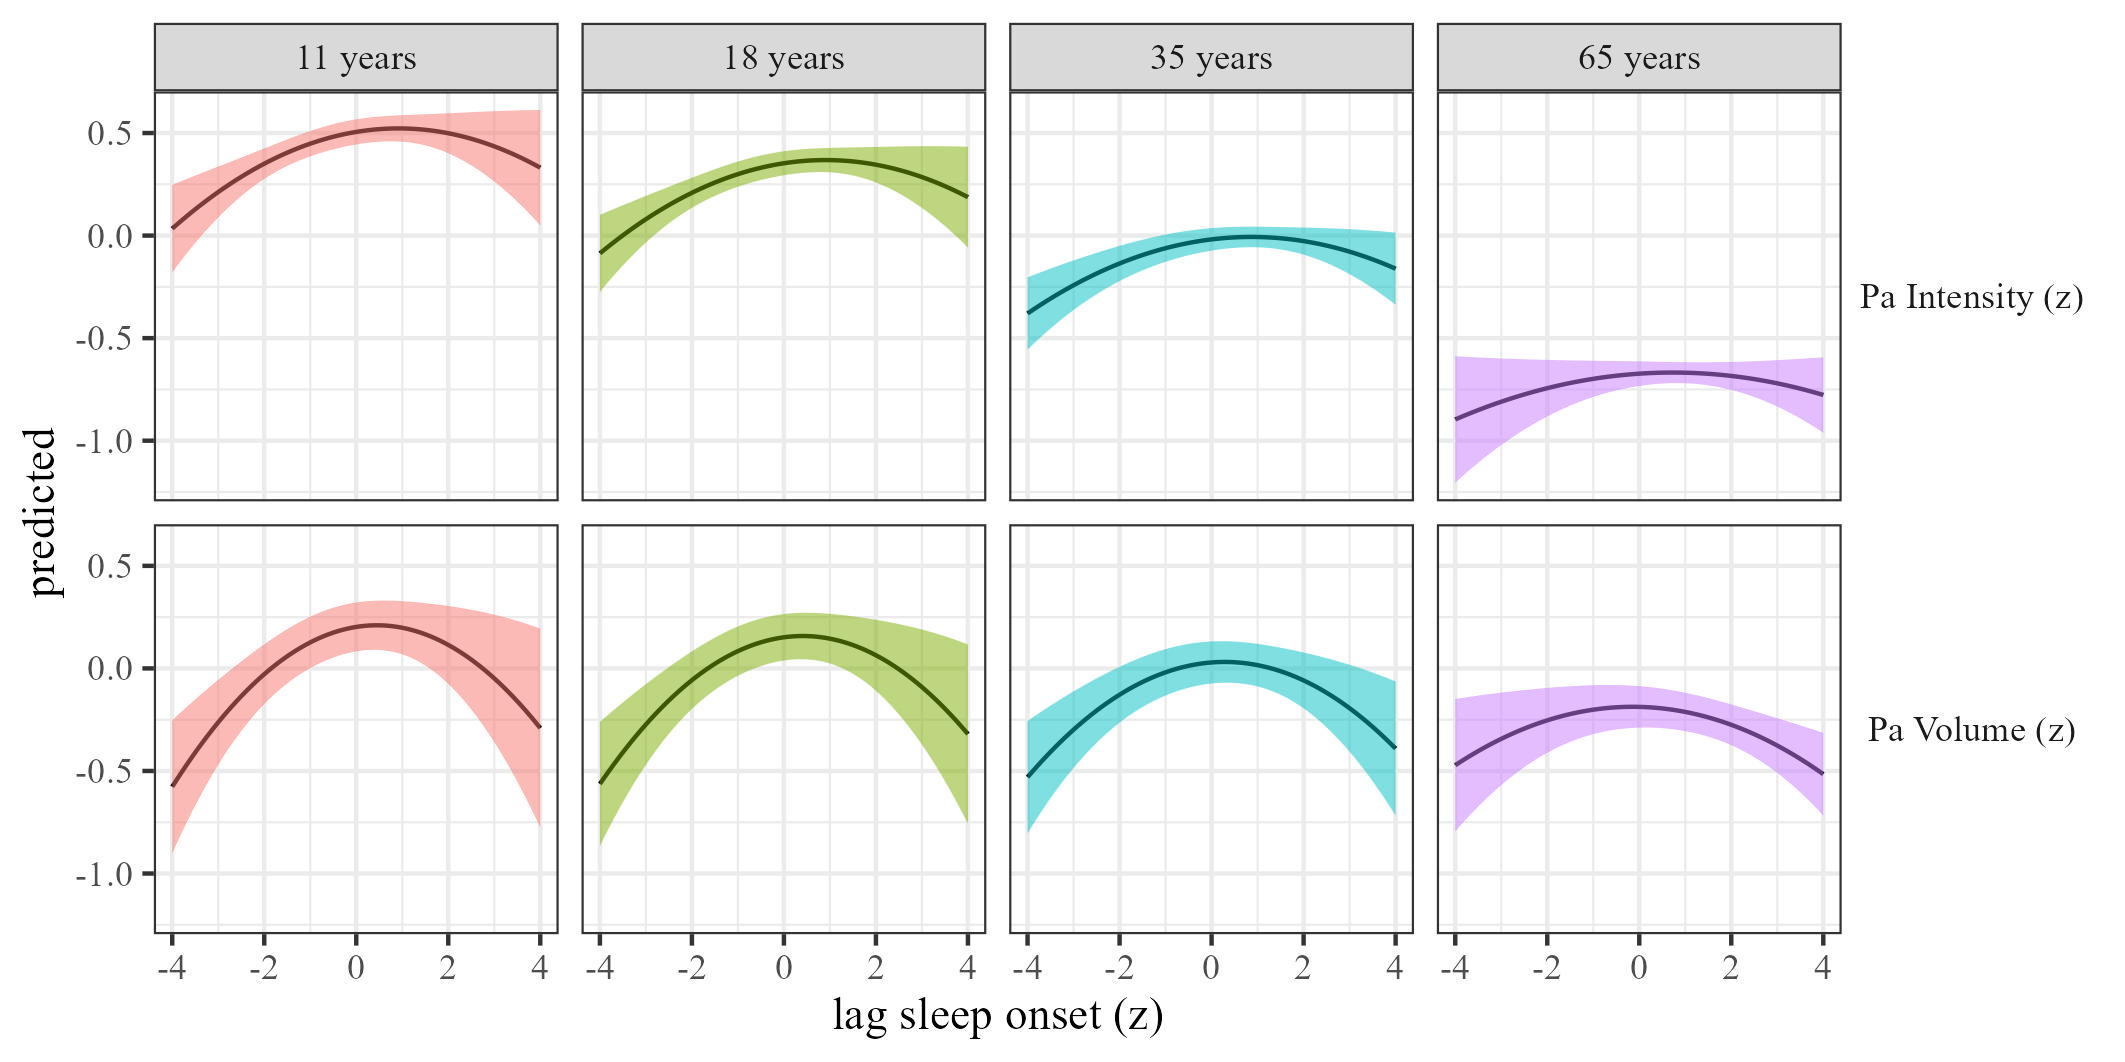
\includegraphics[width=1.1\linewidth]{../Figures/Pa on sleep_onset_lag} \caption{Physical activty by sleep onset}\label{fig:PA-by-sleep-onset-fig}
\end{figure}

\hypertarget{the-effects-of-sleep-regularity-on-physical-activity}{%
\subsection{The effects of sleep regularity on physical activity}\label{the-effects-of-sleep-regularity-on-physical-activity}}

We estimated the effect of sleep regularity on physical activity by age. Results, controlling for sex, SES, and BMI are presented in Table \ref{tab:PA-by-sleep-regularity} and Figure \ref{fig:PA-by-sleep-regularity-fig}. There was a U-shaped relationship between sleep regularity and physical activity volume. Participants with below-average sleep regularity tended to have average physical activity volume. Increases in regularity above the average were linked to greater physical activity volume. There was a strong linear relationship between sleep regularity and physical activity intensity which slightly attenuated with age. Greater sleep regularity was associated with greater physical activity the following day.

\begin{table}[tbp]

\begin{center}
\begin{threeparttable}

\caption{\label{tab:PA-by-sleep-regularity}Physical activity by sleep regularity controlling for SES, gender and BMI}

\begin{tabular}{lllll}
\toprule
Term & \multicolumn{1}{c}{$\beta$ [95\% CI]} & \multicolumn{1}{c}{SE} & \multicolumn{1}{c}{t} & \multicolumn{1}{c}{p}\\
\midrule
PA volume &  &  &  & \\
\ \ \ (Intercept) & 0.38 [-0.02, 0.79] & 0.21 & 1.84 & .191\\
\ \ \ Scale sleep regularity lag & 0.20 [0.17, 0.23] & 0.02 & 12.05 & < .001\\
\ \ \ Age & -0.01 [-0.01, -0.01] & 0.00 & -6.06 & .008\\
\ \ \ Scale sleep regularity lag$^2$ & 0.03 [0.02, 0.04] & 0.01 & 4.32 & < .001\\
\ \ \ Scale sleep regularity lag:age & 0.00 [0.00, 0.00] & 0.00 & -5.07 & .001\\
\ \ \ Age:scale sleep regularity lag$^2$ & 0.00 [0.00, 0.00] & 0.00 & -1.31 & .242\\
PA intensity &  &  &  & \\
\ \ \ (Intercept) & 0.98 [0.59, 1.38] & 0.20 & 4.87 & .035\\
\ \ \ Scale sleep regularity lag & 0.11 [0.09, 0.13] & 0.01 & 10.15 & < .001\\
\ \ \ Age & -0.02 [-0.03, -0.02] & 0.00 & -19.24 & .001\\
\ \ \ Scale sleep regularity lag$^2$ & 0.01 [-0.01, 0.02] & 0.01 & 0.85 & .421\\
\ \ \ Scale sleep regularity lag:age & 0.00 [0.00, 0.00] & 0.00 & -4.01 & < .001\\
\ \ \ Age:scale sleep regularity lag$^2$ & 0.00 [0.00, 0.00] & 0.00 & -0.12 & .903\\
\bottomrule
\addlinespace
\end{tabular}

\begin{tablenotes}[para]
\normalsize{\textit{Note.} Adjusted for SES, BMI, and sex. }
\end{tablenotes}

\end{threeparttable}
\end{center}

\end{table}

\begin{figure}
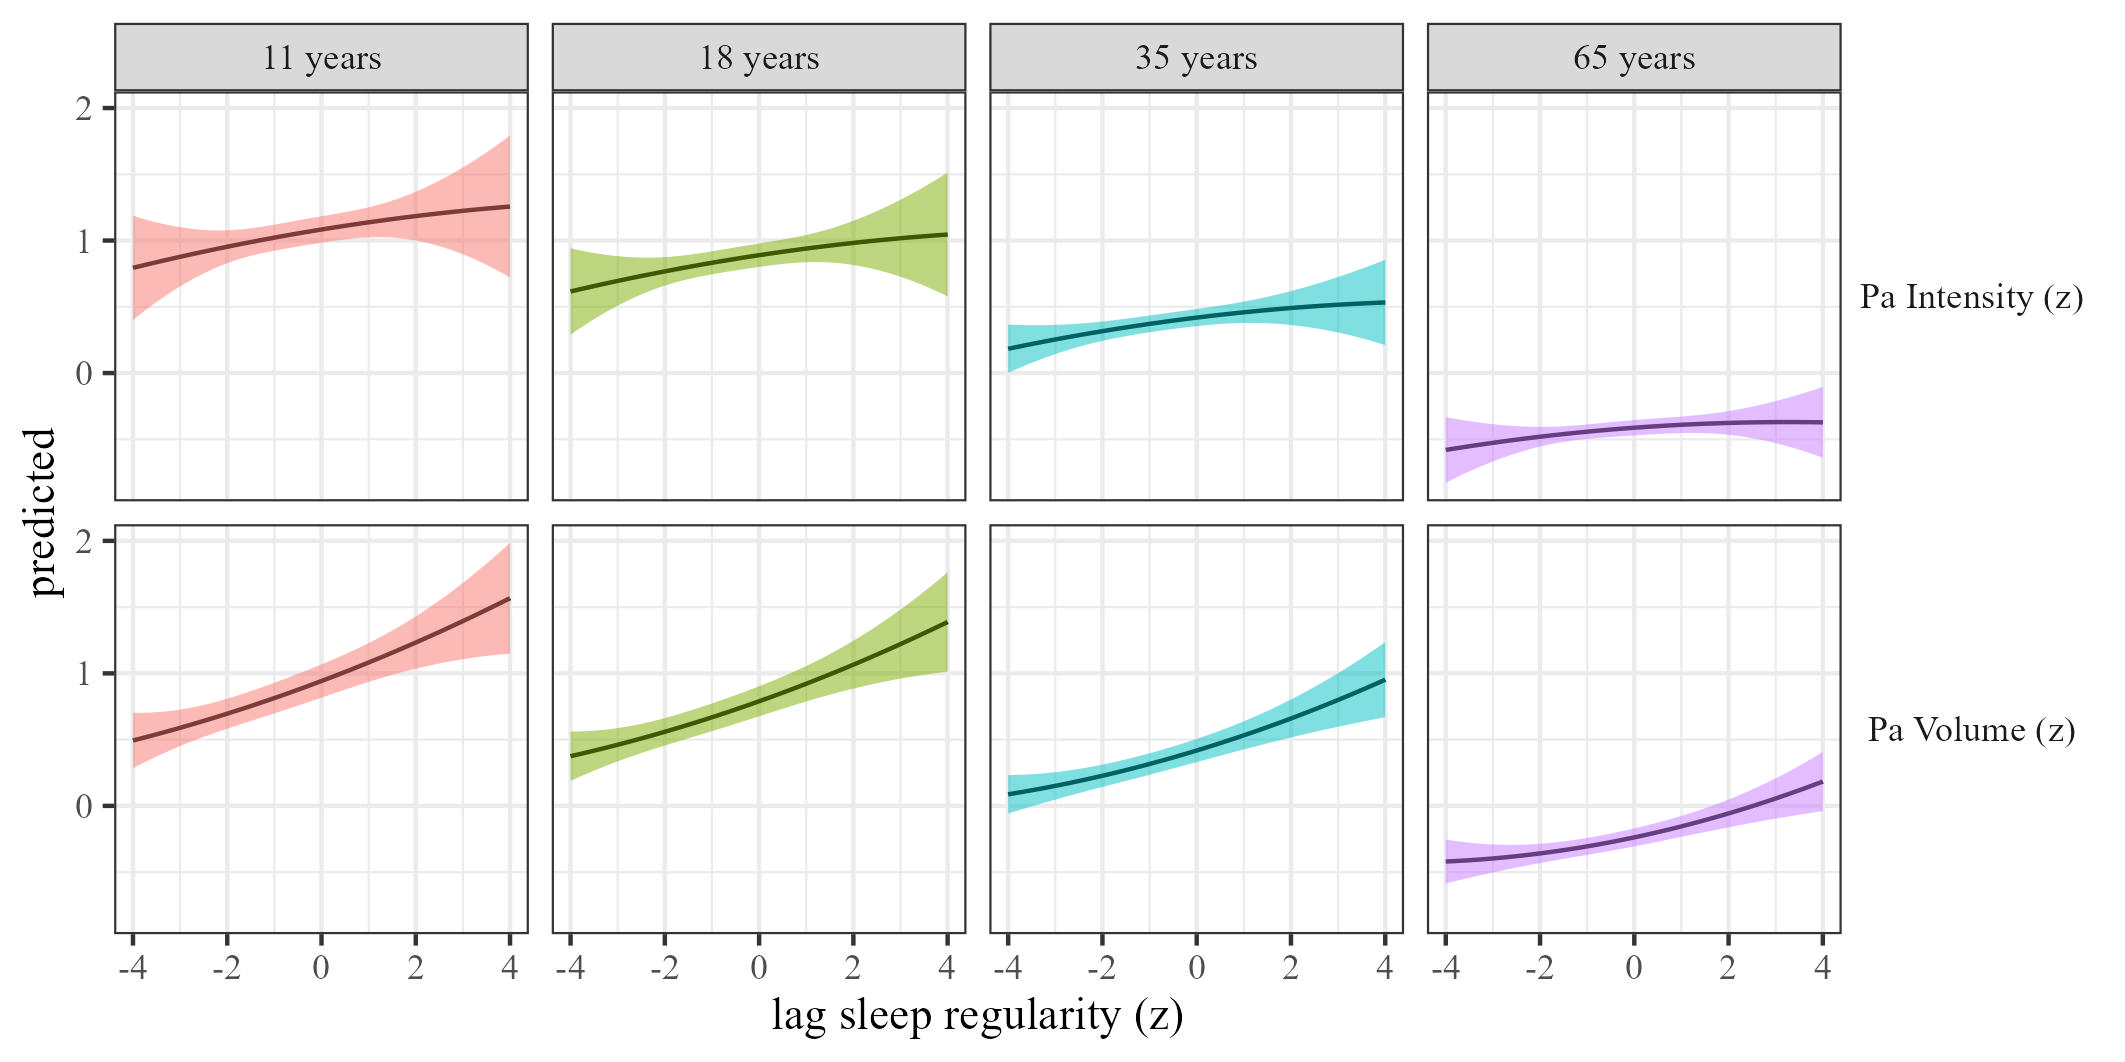
\includegraphics[width=1.1\linewidth]{../Figures/Pa on sleep_regularity_lag} \caption{Physical activty by sleep regularity}\label{fig:PA-by-sleep-regularity-fig}
\end{figure}


\end{document}
